%%This is a very basic article template.
%%There is just one section and two subsections.
\documentclass[parskip=full]{scrartcl}
\usepackage[table]{xcolor}

\usepackage{amsmath}
\usepackage{amsfonts}
\usepackage{mathtools}
\usepackage{studarbeit}
\usepackage{graphicx}
\usepackage{wrapfig}
\usepackage{lscape}
\usepackage{rotating}
\usepackage{epstopdf}
\usepackage{pdfpages}
\usepackage{caption, booktabs}
\usepackage{tabularx}
\usepackage{multirow}
\usepackage{here}
\usepackage[binary-units=true]{siunitx}
 \usepackage[autostyle=true,german=quotes]{csquotes}
 \usepackage{longtable, booktabs}
 \newcommand{\swtLabel}[1]{\textbf{/#1\arabic*0/}}
 \newlist{itemMinus}{itemize}{1 }
 \setlist[itemMinus]{label=--}
  \newlist{itemPlus}{itemize}{1 }
 \setlist[itemPlus]{label=+}
  \newlist{itemPackage}{itemize}{1 }
 \setlist[itemPackage]{label=*}
  \newlist{itemClass}{itemize}{1 }
 \setlist[itemClass]{label=~}
 \newlist{itemClassSub}{itemize}{1 }
 \setlist[itemClassSub]{label=~}
\newlist{itemChange}{itemize}{1 }
 \setlist[itemChange]{label=>}
  \newcommand{\changeDescription}[1]{#1}
 \begin{document}

\title{Elipse -- Einteilungs Interface für das PSE}
\author{D. Biester, E. Dohse, P. Faller, P. Loth, L. Seufert, S. Kopmann}
\thesistype{Implementierungsdokument}
\zweitgutachter{}
\betreuer{Dipl.-Inform.~Andreas~Zwinkau, M.Sc.~Andreas~Fried}
\coverimage{ElipseLogo.png}
\mytitlepage
{\setlength{\textheight}{297mm}
\tableofcontents

\setlength{\textheight}{297mm}}
\pagebreak

\section{Einleitung}

Nachdem im Pflichtenheft beschrieben wurde, was das Produkt leisten soll und
das Entwurfsdokument beantwortete  wie das Produkt strukturiert sein soll, 
beschreibt dieses Dokument nun die Implementierung also die Umsetzung der beiden vorherigen Dokumente.

\section{Implementierungsplan}
Zu beginn der Implementierungsphase wurde ein Plan erstellt, der unser
vorgesehenes Vorgehen beschreibt.
%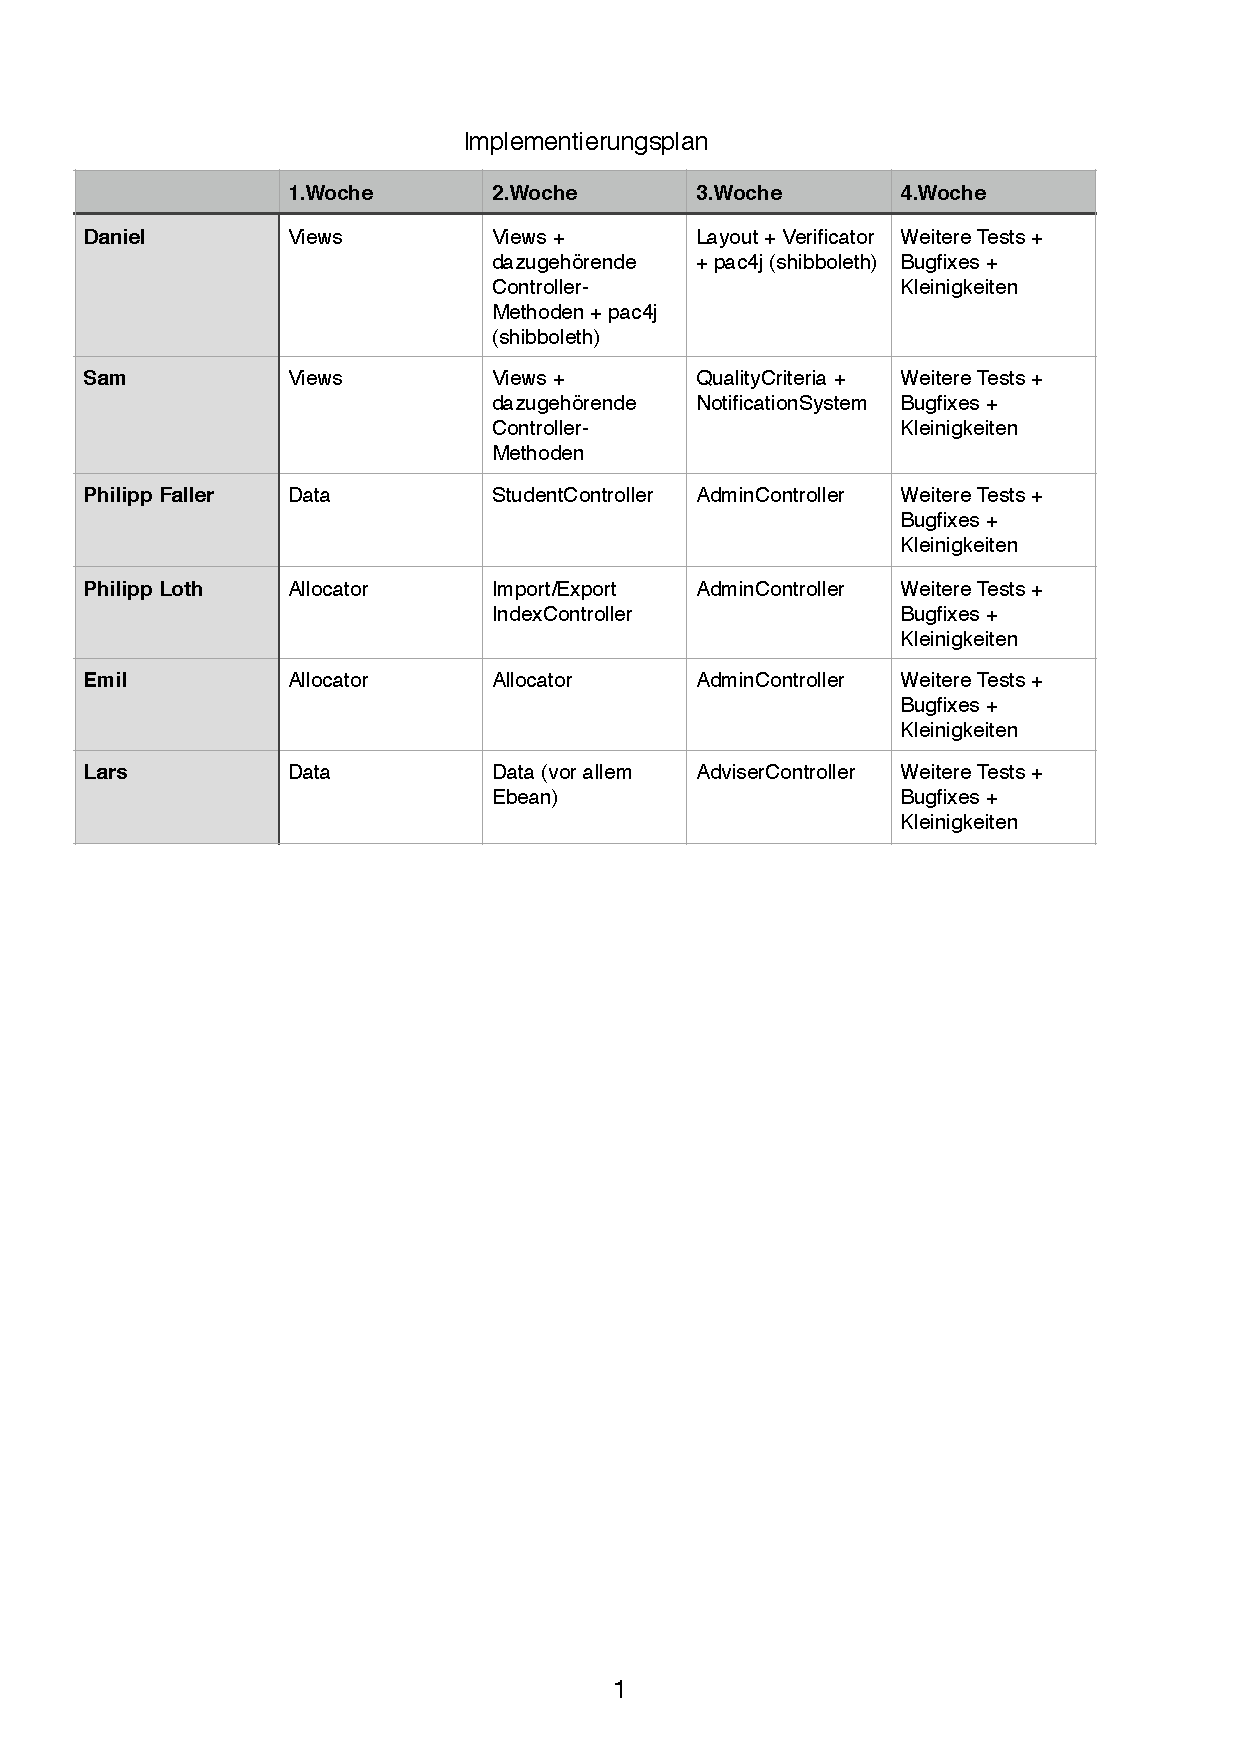
\includepdf[pages={1}]{Implementierungsplan.pdf}

\begin{table}[H]
\begin{tabularx}{\textwidth}{|l|l|X|X|X|}
\hline
 	& 1. Woche			& 2. Woche		& 3. Woche & 4. Woche\\
\hline 
Daniel	& Views			& Views + dazu-gehörende Controller-Methoden + pac4j 
(shibboleth) & Layout + Verificator
+ pac4j (shibboleth)& Weitere Tests +
Bugfixes +
Kleinigkeiten\\
\hline
Sam & Views&Views +
dazu-gehörende
Controller-
Methoden & QualityCriteria +
NotificationSystem & Weitere Tests +
Bugfixes +
Kleinigkeiten\\
\hline
Philipp Faller&Data&Import/Export
IndexController&AdminController&Weitere Tests +
Bugfixes +
Kleinigkeiten\\
\hline
Philipp Loth&Allocator&Import/Export
IndexController&AdminController&Weitere Tests +
Bugfixes +
Kleinigkeiten\\
\hline
Emil&Allocator&Allocator&AdminController&Weitere Tests +
Bugfixes +
Kleinigkeiten\\
\hline
Lars&Data&Data (vor allem
Ebean)&AdviserController&Weitere Tests +
Bugfixes +
Kleinigkeiten\\
\hline
\end{tabularx}
\caption{Implementierungsplan}
\end{table}
% Hierbei war der für uns \enquote{kritische Pfad} %TODO Was ist unser Criticall
% % Path 
% das das Datenmodell gefolgt von paralell implementierbaren Controllern die nur
% auf das Datenmodell zugreiffen und der Allocation. 
Mit sechs Entwicklern in der kurzen Zeit von nur 4 Wochen, die auch noch in der
Prüfungsphase liegt, ein Software-Produkt zu implementieren erfordert, dass die
Entwickler effizient arbeiten können. Da sich jeder von uns bereits in der
Entwurfsphase auf ein Gebiet spezialisiert hatte bot es sich an jedem auf seinem
\enquote{Fachgebiet} auch die Implementierung zu übertragen. 
Ein weiterer Grund für unser Vorgehen war, das wir den Aufwand für
Web-Entwicklung und die Arbeit mir vielen Libraries und Frameworks 
%also das implementieren der Views und deren Anbindung an die Controller und das
% verwenden von ORM-Tools
nicht einschätzen konnten. Daher
wollten wir hier frühzeitig ein funktionierendes Grundgerüst schaffen.
Genau diese herangehensweise bewährte sich, da die Arbeit mit eBean (unserem
ORM-Tool) und dem Play-Framework sich als weit anstrengender herausstellte als
gedacht. Veraltete und nicht vorhandene Dokumentatonen, leer implementerte
Methoden und den guten Ratschlag bei StackOverflow die doch
lieber Hibernate zu verwenden waren allgegenwärtig.


Bei der 
%TODO zweites Diagramm wie haben wir wirklich implementeirt

%dann fairness bzw hierzu nur einen satz aber allgemeine statistiken 


\begin{table}[H]
\begin{tabularx}{\textwidth}{|l|l|X|X|X|}
\hline
 	& 1. Woche			& 2. Woche		& 3. Woche & 4. Woche\\
\hline 
Daniel	& Views			& Views + dazu-gehörende Controller-Methode & Layout + Verificator
+ pac4j&Deadlines + Bugfixes +
Kleinigkeiten \\
\hline
Sam & Views&Views& QualityCriteria +
NotificationSystem & Weitere Tests +
Bugfixes +
Kleinigkeiten\\
\hline
Philipp Faller&Data&Datens&Bugfixes&Bugfixes +  Email\\
\hline
Philipp Loth&Allocator&Import/Export
&Import/Export + Kleinigkeiten &Weitere Tests +
Bugfixes +
Form Validation\\
\hline
Emil&Allocator&Controller&Controller&Form Validation +
Bugfixes +
Kleinigkeiten\\
\hline
Lars&Data&Data (vor allem
Ebean)&Controller + Daten &
Controler-Bugfixes +
Kleinigkeiten\\
\hline
\end{tabularx}
\caption{Wirkliche Implementierung}
\end{table}
\section{Änderungen zum Entwurfsdokument}
Zur Sicherung bessere Code-Qualität (z.B. dem Vermeiden von Code-Copy-Pasting)
und maßgeblich durch die oben beschriebenen Probleme mit verschiedenen
verwendeten Bibliotheken  wurden Änderungen im Vergleich zum  Entrurfsdokument
vorgenommen:
\begin{itemPackage}
\item allocation
\begin{itemClass}
\item Abstract Allocator
\begin{itemClassSub}
\item Methoden
\begin{itemPlus}
\item cancel() 
\item init(Configuration)
\end{itemPlus}
\begin{itemChange}
\item calculate()
\end{itemChange}
\end{itemClassSub}
\item AllocationQueue
\begin{itemClassSub}
\item Methoden
\begin{itemPlus}
\item clear()
\item getAllocator() : AbstractAllocator
\end{itemPlus}
\begin{itemChange}
\item cancelAllocation(String)
\end{itemChange}
\item Attribute
\begin{itemPlus}
\item allocator : AbstractAllocator
\end{itemPlus}
\end{itemClassSub}
\item Configuration
\begin{itemClassSub}
\item Methoden
\begin{itemPlus}
\item getTeams() : List<Team>
\end{itemPlus}
\begin{itemMinus}
\item getProjects() : List<Project>
\end{itemMinus}
\item Konstruktoren
\begin{itemPlus}
\item Configuration(String, List<Student>, List<LearningGroup>, List<Project>,
List<AllocationParameter>)
\end{itemPlus}
\item Atribute
\begin{itemPlus}
\item +teams : List<Team>
\end{itemPlus}
\begin{itemMinus}
\item -projects : List<Project>
\end{itemMinus}
\end{itemClassSub}
\item Criterion
\begin{itemClassSub}
\item Methoden
\begin{itemPlus}
\item getDisplayName(String) : String
\end{itemPlus}
\end{itemClassSub}
\item GurobiAllocator
\begin{itemClassSub}
\item Parameter
\begin{itemPlus}
\item currentConfiguration : Configuration
\end{itemPlus}
\end{itemClassSub}
\item GurobiCriterion
\begin{itemClassSub}
\item Methoden
\begin{itemChange}
\item useCriteria(Configuration, GurobiAllocator, double)
\end{itemChange}
\end{itemClassSub}
\end{itemClass}
\item controller
\begin{itemClass}
\item AdminEditAllocationController
\begin{itemClassSub}
\item Methoden
\begin{itemPlus}
\item editAllocation() : Result
\end{itemPlus}
\begin{itemChange}
\item moveStudents(DynamicForm, List<Integer>) : Result
\item swapStudents(DynamicForm, List<Integer>) : Result
\end{itemChange}
\end{itemClassSub}
\item AdminImportExport
\item \begin{itemClassSub}
\item Methoden
\begin{itemPlus}
\item importGeneral() : Result
\item exportGrades() : Result
\end{itemPlus}
\end{itemClassSub}
\item AdminPageController
\item \begin{itemClassSub}
\item Methoden
\begin{itemPlus}
\item accountPage() : Result
\item notAllowedInCurrentState(String) : Result
\end{itemPlus}
\begin{itemChange}
\item projectEditPage(int) : Result
\end{itemChange}
\end{itemClassSub}
\item AdminPropertiesController
\item \begin{itemClassSub}
\item Methoden
\begin{itemPlus}
\item changeSPO() : Result
\item editSMTPOptions() : Result
\end{itemPlus}
\begin{itemMinus}
\item removeAchievement() : Result
\end{itemMinus}
\end{itemClassSub}
\item AdviserPageController
\item \begin{itemClassSub}
\item Methoden
\begin{itemPlus}
\item notAllowedInCurrentState(String) : Result
\end{itemPlus}
\end{itemClassSub}
\item GeneralAdminController
\item \begin{itemClassSub}
\item Methoden
\begin{itemPlus}
\item removeAllocationFromQueue() : Result
\item editAccount() : Result
\end{itemPlus}
\end{itemClassSub}
\item IndexPageController
\item \begin{itemClassSub}
\item Methoden
\begin{itemPlus}
\item notAllowedInCurrentState(String) : Result
\item passwordResetForm() : Result
\item resetPassord(String) : Result
\end{itemPlus}
\begin{itemMinus}
\item login() : Result
\item passwordReset() : Result
\end{itemMinus}
\end{itemClassSub}
\item MoveStudentCommand
\begin{itemClassSub}
\item Konstruktoren
\begin{itemPlus}
\item MoveStudentCommand(Allocation, List<Student>, Team)
\end{itemPlus}
\item Attribute
\begin{itemPlus}
\item oldTeams : Map<Student, Team>
\item students : List<Student>
\end{itemPlus}
\begin{itemMinus}
\item oldTeam : Team
\item student : Student
\end{itemMinus}
\end{itemClassSub}
\item StudentPageController
\item \begin{itemClassSub}
\item Methoden
\begin{itemPlus}
\item changeData() : Result
\item changeFormPage() : Result
\item notAllowedInCurrentState(String) : Result
\item sendNewVerificationLink() : Result
\item setLearningGroup() : Result
\end{itemPlus}
\end{itemClassSub}
\item SwapStudent
\begin{itemPlus}
\item SwapStudentCommand(Allocation, Student, Student)
\end{itemPlus}
\end{itemClass}
\item data
\begin{itemClass}
\item Administrator
\begin{itemize}
  \item Klasse hinzugefügt
\end{itemize}
\item ElipseModel
\begin{itemize}
  \item Klasse hinzugefügt
\end{itemize}
\item Grade
\begin{itemize}
  \item Enum hinzugefügt
\end{itemize}
\item Transaction
\begin{itemize}
  \item Interface hinzugefügt
\end{itemize}
\item Achievement
\begin{itemClassSub}
\item Methoden
\begin{itemPlus}
\item compareTo(Achievement) : int
\end{itemPlus}
\item Konstruktoren
\begin{itemPlus}
\item Achievement(String)
\end{itemPlus}
\end{itemClassSub}
\item Adviser
\item \begin{itemClassSub}
\item Methoden
\begin{itemPlus}
\item getProjects(): List<Project>
\end{itemPlus}
\begin{itemMinus}
\item addProject(Project)
\item removeProject(Project)
\end{itemMinus}
\item Konstruktoren
\begin{itemPlus}
\item Adviser(String, String, String, String)
\end{itemPlus}
\end{itemClassSub}
\item Allocation
\item \begin{itemClassSub}
\item Methoden
\begin{itemPlus}
\item getSemester() : Semester
\item setSemester(Semester)
\item getTeam(Student) : Team
\item setStudentsTeam(Student, Team)
\item getTeamsByAdviser(Adviser) : List<Team>
\item getTeamsByProject(Project) : List<Project>
\item getNotAllocatedStudents() : List<Student>
\end{itemPlus}
\begin{itemMinus}
\item clone() : Allocation
\end{itemMinus}
\item Konstruktoren
\begin{itemPlus}
\item Allocation(List<Team>, String, List<AllocationParameter>)
\item Allocation(Allocation)
\end{itemPlus}
\item Attribute
\begin{itemPlus}
\item semester : Semester
\end{itemPlus}
\end{itemClassSub}
\item AllocationParameter
\begin{itemClassSub}
\item Konstruktoren
\begin{itemPlus}
\item AllocationParameter(String, int)
\end{itemPlus}
\end{itemClassSub}
\item GeneralData
\begin{itemClassSub}
\item Methoden
\begin{itemPlus}
\item loadInstance() : GeneralData
\end{itemPlus}
\begin{itemMinus}
\item getAdminName() : String
\item setAdminName(String)
\item getAdminPassword() : String
\item setAdminPassword(String)
\end{itemMinus}
\item Attribute 
\begin{itemMinus}
\item adminName : String
\item adminPassword : String
\end{itemMinus}
\end{itemClassSub}
\item LearningGroup
\begin{itemClassSub}
\item Methoden
\begin{itemPlus}
\item getSemester() : Semester
\item setSemester(Semester)
\item addMember(Student)
\item removeMember(Student)
\end{itemPlus}
\item Konstruktoren
\begin{itemPlus}
\item LearningGroup(String, String)
\item LearningGroup(String, String, Student, boolean)
\end{itemPlus}
\item Attribute 
\begin{itemPlus}
\item semester : Semester
\end{itemPlus}
\end{itemClassSub}
\item Project
\begin{itemClassSub}
\item Methoden
\begin{itemPlus}
\item setSemester(Semester)
\item getSemester() : Semester
\item addAdviser(Adviser)
\item removeAdviser(Adviser)
\end{itemPlus}
\begin{itemMinus}
\item getRating(Student) : int
\item getProject(String, Semester) : Project
\end{itemMinus}
\item Konstruktoren
\begin{itemPlus}
\item Project(String, String, String, String)
\item Project(String, Adviser)
\end{itemPlus}
\item Attribute 
\begin{itemPlus}
\item semester : Semester
\end{itemPlus}
\end{itemClassSub}
\item Rating
\begin{itemClassSub}
\item Methoden
\begin{itemPlus}
\item getLearningGroup() : LearningGroup
\item setLearningGroup(LearningGroup)
\end{itemPlus}
\item Konstruktoren
\begin{itemPlus}
\item Rating(int, Project)
\end{itemPlus}
\item Attribute 
\begin{itemPlus}
\item learningGroup : LearningGroup
\end{itemPlus}
\end{itemClassSub}
\item Semester
\begin{itemClassSub}
\item Methoden
\begin{itemPlus}
\item getMaxGroupSize() : int
\item setMaxGroupSize(int)
\item isWintersemester() : boolean
\item setWintersemester(boolean)
\item addAllocation(Allocation)
\item removeAllocation(Allocation)
\item addProject(Project)
\item removeProject(Project)
\item addStudent(Student)
\item removeStudent(Student)
\item addLearningGroup(LearningGroup)
\item removeLearningGroup(LearningGroup)
\item addSPO(SPO)
\item removeSPO(SPO)
\item getLearningGroupOf(Student) : LearningGroup
\item compareTo(Semester) : int
\end{itemPlus}
\item Konstruktoren
\begin{itemPlus}
\item Semester(String, boolean)
\end{itemPlus}
\item Attribute 
\begin{itemPlus}
\item wintersemester : boolean
\item maxGroupSize : int
\end{itemPlus}
\end{itemClassSub}
\item SPO
\begin{itemClassSub}
\item Methoden
\begin{itemPlus}
\item addAdditionalAchievement(Achievement)
\item removeAdditionalAchievement(Achievement)
\item addNecessaryAchievement(Achievement)
\item removeNecessaryAchievement(Achievement)
\item compareTo(SPO) : int
\item equals(Object) : boolean
\end{itemPlus}
\item Konstruktoren
\begin{itemPlus}
\item SPO(String)
\end{itemPlus}
\end{itemClassSub}
\item Student
\begin{itemClassSub}
\item Methoden
\begin{itemPlus}
\item toStringForNotification() : String
\item registeredMoreThanOnce() : boolean
\end{itemPlus}
\begin{itemMinus}
\item getRating(Project) : int
\item setRating(Project, int)
\item getCurrentProject() : Project
\item getCurrentTeam() : Team
\end{itemMinus}
\item Konstruktoren
\begin{itemPlus}
\item Student(String, String, String, String, String, int, SPO,
List<Achievement>, List<Achievement>, int)
\end{itemPlus}
\item Attribute 
\begin{itemChange}
\item gradePSE : Grade
\item gradeTSE : Grade
\end{itemChange}
\end{itemClassSub}
\item Team
\begin{itemClassSub}
\item Methoden
\begin{itemPlus}
\item getAllocation() : Allocation
\item setAllocation(Allocation)
\item getTeamNumber() : int
\item setTeamNumber(int)
\item addMember(Student)
\item removeMember(Student)
\item toStringForNotification() : String
\end{itemPlus}
\begin{itemMinus}
\item getRating(Student) : int
\end{itemMinus}
\item Konstruktoren
\begin{itemPlus}
\item Team(Project, List<Student>)
\end{itemPlus}
\item Attribute 
\begin{itemPlus}
\item teamNumber : int
\item allocation : Allocation
\end{itemPlus}
\end{itemClassSub}
\item User
\begin{itemClassSub}
\item Methoden
\begin{itemPlus}
\item compareTo(User) : int
\end{itemPlus}
\item Konstruktoren
\begin{itemPlus}
\item User(String, String, String, String, String)
\end{itemPlus}
\end{itemClassSub}
\end{itemClass}
\item deadline
	\begin{itemClass}
	\item DeadLineFilter
	\begin{itemize}
	  \item Klasse hinzugefügt
	\end{itemize}
	\item StateStorage
	\begin{itemize}
	  \item Klasse hinzugefügt
	\end{itemize}
	\end{itemClass}
\item exception
\begin{itemClass}
\item DataException
\begin{itemize}
	  \item Klasse hinzugefügt
	\end{itemize}
\item ImporterException
\begin{itemize}
	  \item Klasse hinzugefügt
	\end{itemize}
\end{itemClass}
\item filters
\begin{itemClass}
\item Filter
\begin{itemize}
	  \item Klasse hinzugefügt
	\end{itemize}
\end{itemClass}
\item importExport
\begin{itemClass}
\item Importer
\begin{itemClassSub}
\item Methoden
\begin{itemPlus}
\item exportGrades(File, Semester)
\end{itemPlus}
\begin{itemMinus}
\item importCMSData(File, Semester)
\item exportCMSData(File, Semester)
\end{itemMinus}
\end{itemClassSub}
\end{itemClass}
\item notificationSystem
\begin{itemClass}
\item Notifier
\begin{itemClassSub}
\item Methoden
\begin{itemPlus}
\item notifyAdviser(Allocation, Adviser)
\item notifyStudent(Allocation, Student)
\item sendAdviserPassword(Adviser, String)
\end{itemPlus}
\item Konstruktoren
\begin{itemPlus}
\item Notifier(MessagesApi)
\end{itemPlus}
\end{itemClassSub}
\end{itemClass}
\item qualityCriteria
\begin{itemClass}
\item QualityCriterion
\begin{itemClassSub}
\item Methoden
\begin{itemPlus}
\item getName(String) : String
\end{itemPlus}
\end{itemClassSub}
\end{itemClass}
\item security
\begin{itemClass}
\item BlowfishPasswordEncoder
	\begin{itemize}
	  \item Klasse hinzugefügt
	\end{itemize}
\item EmailVerifier
\item \begin{itemize}
	  \item Klasse hinzugefügt
	\end{itemize}
\item PasswordResetter
\item \begin{itemize}
	  \item Klasse hinzugefügt
	\end{itemize}
\item SecurityModule
\begin{itemClassSub}
\item Konstruktoren
\begin{itemPlus}
\item SecurityModule(Enviroment, Configuration)
\end{itemPlus}
\end{itemClassSub}
\item TimedCodeValueStore
\item \begin{itemize}
	  \item Klasse hinzugefügt
	\end{itemize}
\item UserAuthentikator
\item \begin{itemize}
	  \item Klasse hinzugefügt
	\end{itemize}
\item UserManagement
\item \begin{itemize}
	  \item Klasse hinzugefügt
	\end{itemize}
\item UserProfile
\item \begin{itemize}
	  \item Klasse hinzugefügt
	\end{itemize}
\item Verifier
\item \begin{itemize}
	  \item Klasse hinzugefügt
	\end{itemize}
\end{itemClass}
\item view
\begin{itemize}
  \item Package hinzugefügt
\end{itemize}
\end{itemPackage}
\subsection{allocation}
\begin{itemize}
  \item 
\end{itemize}

\section{Funktionsumfang}
Wie im Pflichtenheft beschrieben gibt es einige Muss und Wunschkriterien zu
diesem Produkt. Ein Großteil dieser wurde von uns Implementiert.
\subsection{Einteilungsfunktionen}
\subsubsection{Pflichtfunktionen}
\begin{enumerate}[label=\swtLabel{FA}]
  \item Einteilung der Studierenden zu Projekten. Hierbei werden folgende Kriterien,
soweit möglich und wie konfiguriert berücksichtigt:
\begin{itemize}
  \item Wer die durch seine SPO gegebenen Voraussetzungen nicht erfüllt, wird nicht
eingeteilt
\item Möglichst viele Studierende werden zu Projekten zugeteilt
\item Lerngruppen bleiben zusammen
\item Projektbewertung der Studierenden werden berücksichtigt
\end{itemize}
\item Berechnung von Gütekriterien
\end{enumerate}
\subsubsection{Wunschfunktionen}
\begin{enumerate}[label=\swtLabel{FA}, resume]
  \item Stapelverarbeitung von mehreren Einteilungen mit unterschiedlichen Konfigurationen
\item Folgende Kriterien fließen in die Einteilung ein:
\begin{itemize}
  \item Wer sich zum zweiten Mal bewirbt, soll bei der Einteilung bevorzugt
  werden
  \item Eher 5er-Teams als 6er-Teams
  \item Studierende in einem Team sind im gleichen Semester
  \item Studierende höheren Semesters werden bevorzugt
  \item Studierende, die bereits mehr Teilleistungen aus dem ersten Jahr bestanden
haben, werden bevorzugt
\end{itemize}
\end{enumerate}
\subsection{Adminfunktionen}

\subsubsection{Pflichtfunktionen}
\begin{enumerate}[label=\swtLabel{FA}, resume]
  \item Anmeldung
  \item Initialisierung des Produktes bestehend aus einer Initialisierung der Datenbank
und des Webservers
\item Setzten der frühest möglichen Anmeldezeit für Studierende
\item Setzen der Projektbewertungsdeadline
\item Einstellen einer Einteilungskonfiguration
\item Starten der Einteilungsberechnung
\item Übersicht über die aktuelle Einteilung
\item Anzeige der Gütekriterien bestehend aus:
\begin{itemize}
  \item Studierenden-Happiness
  \item Anzahl der nicht zugeteilten Studierenden
  \item Anzahl der getrennten Lerngruppen
\end{itemize}
\item Studierende aus dem Produkt entfernen
\item Studierende zum Produkt hinzufügen
\item Studierende zu einem Team bei einer bereits berechneten Einteilung
hinzufügen
\item Studierende von einem Team bei einer bereits berechneten Einteilung
entfernen
\item Studierende zwischen Teams bei einer bereits berechneten Einteilung verschie-
ben
\item Import von Einteilungs-, SPO- und Studierendendaten
\item Export von Einteilungs-, SPO- und Studierendendaten
\item Erstellung eines Projektes
\item Ändern der Projektdetails: Name, Beschreibung, Projektbetreuer, minimale
und maximale Teilnehmerzahl, der Teams
\item Löschen eines Projektes
\item Abmeldung
\item Finale Wahl und Veröffentlichung einer Einteilung
\end{enumerate}
\subsubsection{Wunschfunktionen}
\begin{enumerate}[label=\swtLabel{FA}, resume]
  \item Abbrechen der Einteilungsberechnung
  \item Hinzufügen von Berechnungen zur Stapelverarbeitung
  \item Hinzufügen wählbarer Teilleistungen zu SPOs
  \item Entfernen wählbarer Teilleistungen aus SPOs
  \item SPOs auswählen, die Studierende bei der Anmeldung angeben können 
\item 
Benachrichtigen der Studierende und Projektbetreuer über die Einteilung
per E-Mail
\item Erstellen von Betreueraccounts unter Angabe der Daten /D310/ bis /D340/
\item Import von „.csv“-Dateien mit Informationen über bestandene Teilleistungen
der Studierenden aus dem Campus Management System
\item Anzeige von Konflikten bei Teilleistungen der Studierenden nach dem Import
vom Campus Management System-Daten
\item Export von „.csv“-Dateien mit Noten der Studierenden
\item Übersicht über bereits berechnete Einteilungen
\item Warnung an den Administrator, falls er bei der manuellen Nachjustierung
der Einteilung die bei der Konfiguration angegebenen Grenzen überschreitet
\end{enumerate}


\subsection{Studierendenfunktionen}
\subsubsection{Pflichtfunktionen}
\begin{enumerate}[label=\swtLabel{FA}, resume]
  \item Registrierung eines Studierenden mit Datenerfassung:
  \begin{itemize}
    \item Vorname, Nachname, Matrikelnummer, E-Mail-Adresse, Semester und Pass-
wort
\item Auswahl bestandener Teilleistungen und der SPO
\item Auswahl noch ausstehender Nachprüfungen
  \end{itemize}
  \item Anmeldung mit Matrikelnummer und Passwort
  \item Projektbewertung der Projekte
  \item Erstellung einer Lerngruppe mit Name und Passwort
  \item Projektbewertung der Projekte für die Lerngruppe
  \item Beitritt zu einer Lerngruppe
  \item Austritt aus einer Lerngruppe
  \item Übersicht der eigenen Lerngruppe
  \item Abmeldung
  \item Einsicht der Einteilungsergebnisse
\end{enumerate}
\subsubsection{Wunschfunktionen}
\begin{enumerate}[label=\swtLabel{FA}, resume]
  \item Anzeigen von Projektbeschreibung in Projektbewertungseingabemaske
  \item Anmeldung über SCC-Account
  \item Verifikation der E-Mail-Adresse über einen Verifikationslink, der an die vom
Studierenden angegebene E-Mail-Adresse versandt wird
\item Anfordern eines neuen Passworts
\end{enumerate}

\subsection{Betreuerfunktionen}
\subsubsection{Wunschfunktionen}
\begin{enumerate}[label=\swtLabel{FA}, resume]
  \item Anmeldung
  \item Erstellung eines Projektes
  \item Ändern der Projektdetails: Name, Beschreibung, Projektbetreuer, minimale
und maximale Teilnehmerzahl, Anzahl der Teams
\item Einsehen der Einteilung zu eigenen Projekten
\item Einsicht, ob zugeteilte Studierende noch Nachprüfungen ausstehen haben
\item Einsicht, ob zugeteilte Studierende schon im Campus Management System für
PSE und TSE angemeldet sind
\item Abmeldung
\item Noteneintragung für Studierende der betreuten Projekte
\item Einem Projekt als Betreuer beitreten
\item Ein Projekt als Projektbetreuer verlassen
\end{enumerate}



%Muss und wunsch

%Tests

%Code Kommentieren nochmal?
\end{document}